%\part{Classical transport}\label{part:1}  # Optional



\chapter{Transport equations}\label{sec:transportequations}
Imagine an infinitely large billiard table.
A particle---represented by the white billiard ball---moves frictionlessly along straight 
lines until undergoing elastic, instantaneous collisions with background 
obstacles---the black billiard balls---that do not move due to their infinite weight and neglectable velocity.
The situation is depicted in
Figure \ref{fig:particlebilliardtable}.

\begin{figure}[h!]
	\centering
	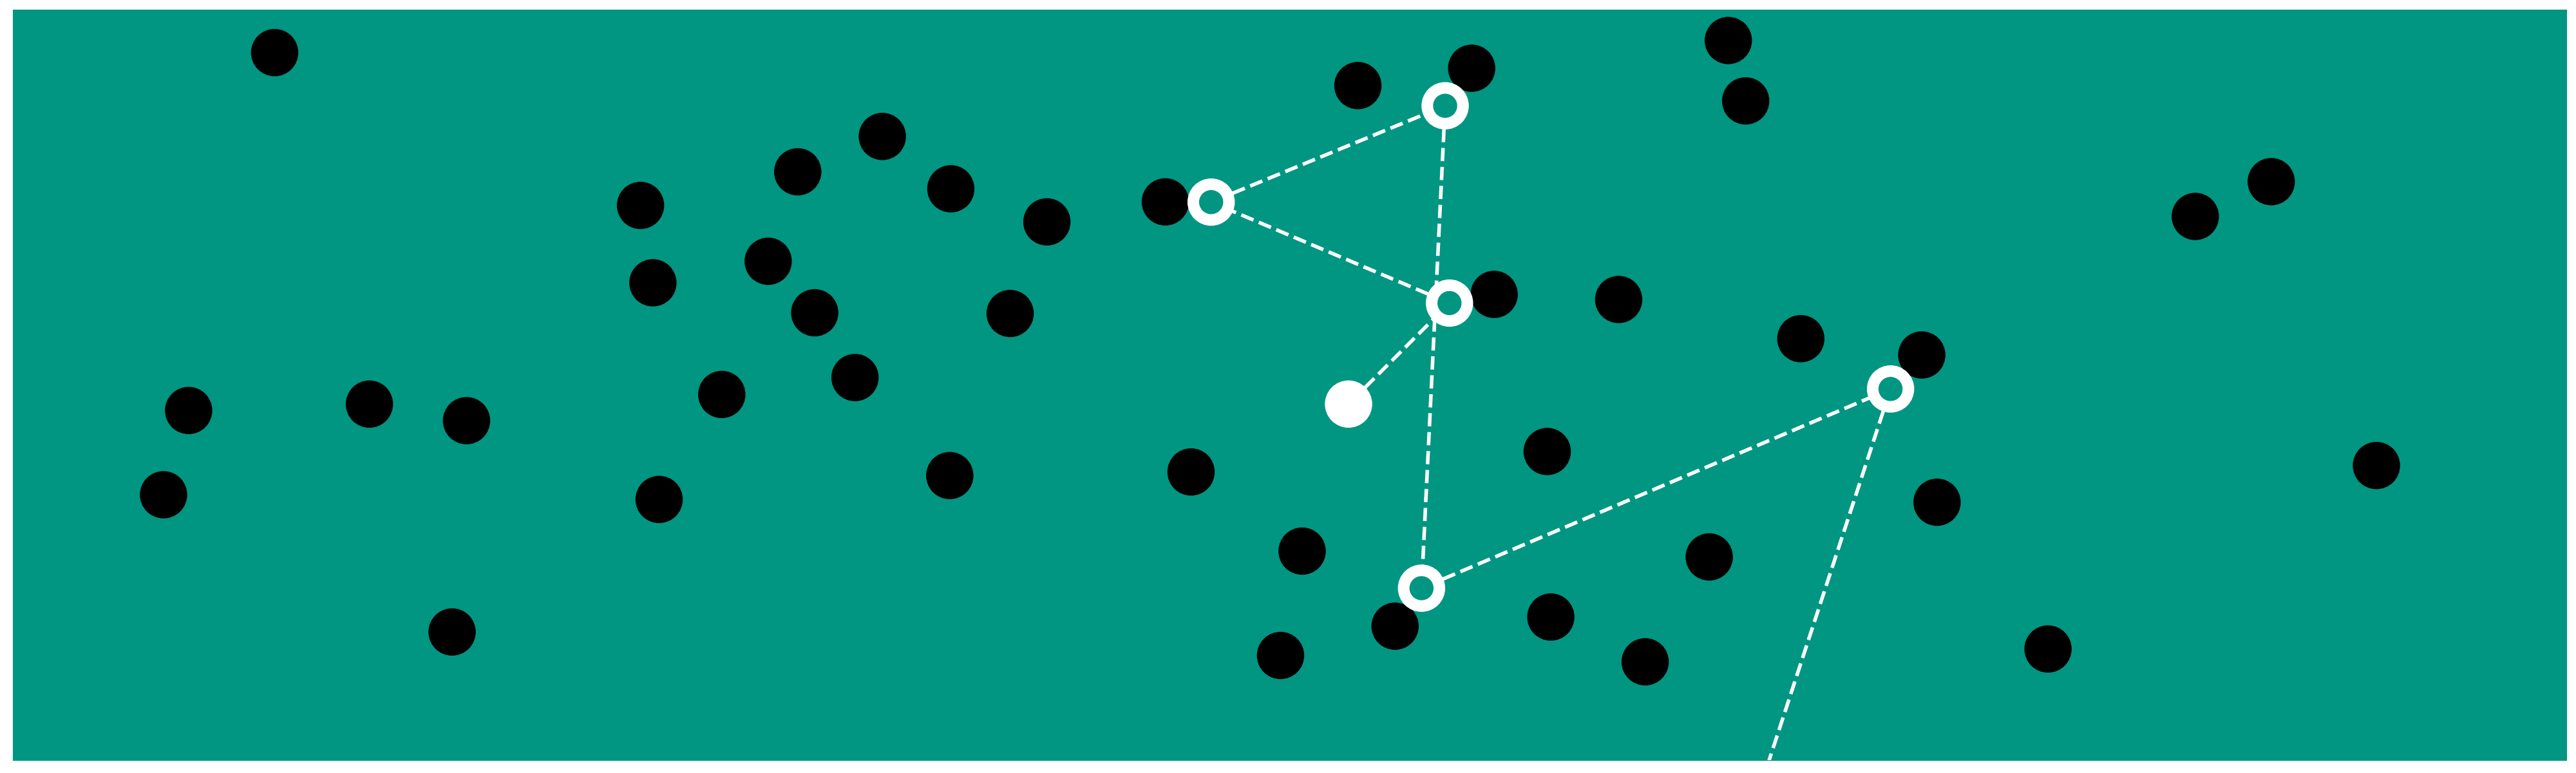
\includegraphics[width=1.0\linewidth]{Chapters/Chapter1/figs/billiardtable/particlebilliardtable}
	\caption{The white ball undergoes elastic collisions on the billiard table while the black balls' positions are fixed.}
	\label{fig:particlebilliardtable}
\end{figure}

This in many ways simplified microscopic description of particle interactions will serve as the 
starting point for this thesis. Despite its simplicity, it allows the derivation of governing 
mesoscopic and macroscopic equations, as well as the construction of one of the most 
prominent numerical methods in transport theory---the Monte Carlo method. Furthermore, 
changing the microscopic picture will motivate non-classical transport, discussed in the 
second part of this thesis.

A magnitude of real-world phenomena and topics can be formulated in the language of kinetic 
theory. These include, but are not limited to, the theory of gases; radiation therapy for cancer 
treatment; modeling of nuclear reactors; or illumination in movies and computer games.

Transport equations try to achieve the following: Instead of describing a 
system by the behavior of every single molecule, every single particle, or every single light-ray, 
they seek a description in terms of statistical quantities that evolve in time. This is both 
necessary and often desirable. Necessary, since it already becomes computationally 
impossible 
to evolve the trajectory of each of the roughly $6.022\cdot 10^{23}$ particles in one mole.
Desirable, since it is generally of no interest to know each of these trajectories individually.
Thus, transport equations are convenient tools that distill complex physical systems to 
manageable equations.


Throughout the scope of this thesis we are going to consider uncharged particle 
transport; 
that is, particles do not interact with another via long range interactions---like electrons 
do---but with the background medium or through direct collisions with another.
Given these assumptions, particles move through phase space according to Newton's laws of motion
\begin{align}
	\begin{cases}
		\dot{\bx}(t) & = \bv(t),                          \\
		\dot{\bv}(t) & = \frac{1}{m} {\bf{F}}(t,\bx(t),\bv(t)), \\
	\end{cases}
	\label{eq:NewtonsLaw}
\end{align}
with $\bx(t),\bv(t) \in \RThree$, $t\in\Rgeqz$, $m\in \Rgz$, ${\bf{F}}: \Rgeqz \times \RThree \times \RThree \to \RThree$ sufficiently smooth, and subject to initial conditions $\bx(0) = \bx_0$ and $\bv(0) = \bv_0$. If we again assume that particles move with a much smaller mass and faster than background obstacles, and if we also neglect particle-particle interactions, it is easy to track particle trajectories through the obstacle field as already seen in  Figure \ref{fig:particlebilliardtable}.


\section{And here starts a new subsection}
With some text.
\subsection{And maybe a new subsection?}
Some more text.
A list of your todos---including the one here---can be found in the beginnig of your thesis. Remove that list before the final publication.\todo{Sometimes you want to write yourself a reminder}

\section{Citations}
You can cite people easily \cite{camminady2017nonclassical}. 




\section{Table}
For different weight functions $w$, some orthogonal polynomials are given in Table
\ref{tab:orthopolys}.


\begin{table}
	\centering
	\begin{tabular}{lcr}
		\toprule
		\hfill Weight function \hfill & Interval           & \hfill Orthogonal polynomials \hfill \\
		\midrule
		$w(x) = 1$                    & $[-1,1]$           & Legendre                             \\ \addlinespace
		$w(x) = 1/\sqrt{1-x^2}$       & $(-1,1)$           & Chebyshev ($1^{\text{st}}$ kind)     \\
		\addlinespace
		$w(x) = \sqrt{1-x^2}$         & $[-1,1]$           & Chebyshev  ($2^{\text{nd}}$ kind)    \\
		\addlinespace
		$w(x) = e^{-x}$               & $[0,\infty)$       & Laguerre                             \\ \addlinespace
		$w(x) = e^{-x^2}$             & $(-\infty,\infty)$ & Hermite                              \\ \addlinespace
		\bottomrule
	\end{tabular}
	\caption{Table of weight functions and corresponding orthogonal polynomials.}
	\label{tab:orthopolys}
\end{table}


\section{Algorithm}


My favorite algorithm is Algorithm \ref{alg:rSN}, not Algorithm \ref{alg:SN}.

\renewcommand{\highlight}[1]{\setlength{\fboxsep}{2pt}\colorbox{kitgreen100!0}{{\color{kitgreen100}$\displaystyle #1$}}}
\newcommand{\fakehighlight}[1]{\setlength{\fboxsep}{2pt}\colorbox{kitgreen100!0}{{$\displaystyle #1$}}}

\begin{minipage}{0.49\textwidth}
	\begin{algorithm}[H]
		\centering
		\caption{The S$_N$ method.}\label{algorithm1}
		\begin{algorithmic}[1]
			\Function{S$_N$}{$\Delta t, t_{\text{end}},\text{order},n_x,\fakehighlight{n_y},\psi_0$ }$\fakehighlight{\color{white}{\delta}}$
			\State $t \gets 0$
			\State $n_q \gets \fakehighlight{\text{order}^2 {\color{white}48}}$ $\fakehighlight{\color{white}{\text{New}}}$
			\State $P \gets\fakehighlight{\text{QPoints}(n_q)$ $\in \mathbb{R}^{3 \times n_q}}$$\fakehighlight{\color{white}{\text{New}}}$
			\State $W\gets\fakehighlight{\text{QWeights}(n_q)$ $\in \mathbb{R}^{n_q}}$
			\State $\psi \gets\psi_0$ $\in \mathbb{R}^{n_q \times n_x \times n_y}$
			\While{$t< t_\text{end}$}
			\State $F \gets \text{ComputeFlux}(\psi,P,W)$
			\State $\psi \gets \psi + \Delta t \cdot F$
			\State $\fakehighlight{\color{white}{\psi,Q \gets \text{RotateInterpolate}(\psi,Q,\delta\cdot \delta t /n_q)}}$
			\State $\fakehighlight{\color{white}{\psi,Q \gets \text{RotateInterpolate}(\psi,Q,\delta\cdot \delta t /n_q)}}$
			\State $t\gets t + \Delta t$
			\EndWhile
			\State \textbf{return} $\psi$
			\EndFunction
		\end{algorithmic}
		\label{alg:SN}
	\end{algorithm}
\end{minipage}
\hfill
\begin{minipage}{0.49\textwidth}
	\begin{algorithm}[H]
		\centering
		\caption{The rS$_N$ method.}
		\label{algorithm1}
		\begin{algorithmic}[1]
			\Function{${}$rS$_N$}{$\Delta t, t_{\text{end}},\text{order},n_x,n_y,\psi_0 , \highlight{\delta}$}
			\State $t \gets 0$
			\State $n_q \gets  \highlight{4\cdot\text{order}^2 - 8\cdot\text{order}+6}$
			\State $P \gets\highlight{\text{NewQPoints}(n_q)$ $\in \mathbb{R}^{3 \times n_q}}$
			\State $W\gets\highlight{\text{NewQWeights}(n_q)$ $\in \mathbb{R}^{n_q}}$
			\State $\psi \gets\psi_0$ $\in \mathbb{R}^{n_q \times n_x \times n_y}$
			\While{$t< t_\text{end}$}
			\State $F \gets \text{ComputeFlux}(\psi,P,W)$
			\State $\psi \gets \psi + \Delta t \cdot F$
			\State $\highlight{\alpha \gets \delta\cdot \Delta t /n_q}$
			\State $\highlight{\psi,P \gets \text{RotateInterpolate}(\psi,P,\alpha)}$
			\State $t\gets t + \Delta t$
			\EndWhile
			\State \textbf{return} $\psi$
			\EndFunction
		\end{algorithmic}
		\label{alg:rSN}
	\end{algorithm}
	
\end{minipage}
